\documentclass[../../main.tex]{subfiles}
\begin{document}

\begin{figure}[t]
	\centering
	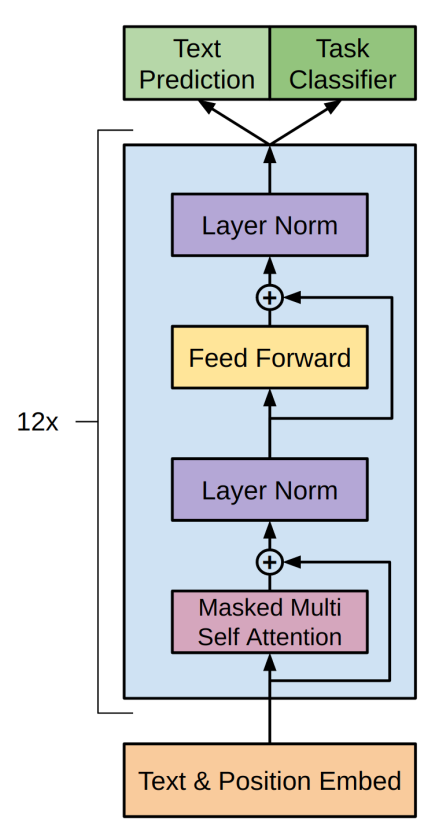
\includegraphics[scale=0.3]{include/images/gpt_architecture.png}
	\caption{
		The GPT archictecture \cite{Radford2018}.
		A transformer encoder
		without connections to a previous encoder is used.
		The attention layer
		can only attend on previous positions in the input sequence.
		The decoder is stacked $12$ times before generating the final output.
	}
	\label{fig:gpt_arch}
\end{figure}

Decoder only transformers make up the base of generative pre-trained transformers (GPT).
The decoder used for GPT does not rely on the outputs of a encoder,
because it designed made for generation tasks.
In Figure \ref{fig:gpt_arch} we can see
that only the masked multi-head attention layer is kept in comparison to
the the full transformer network.
The simple archticture enables faster pre-training and fine-tuning.

GPT is trained in two phases.
In the unsupervised pre-training phase,
the model is trained with big datasets of unlabed text data.
The training objective here is
to accurataly generate the next token of a sequence.

After the first pre-training phase,
the model needs to be fine-tuned a for a specific task.
By including custom tokens in the fine-tuning dataset,
the decoder can learn to handle a variety of different tasks
such as text generation or classification.

Newer research on generation models focuses on scaling the network.
The \textit{scaling law} states
that by simply increasing the amount of parameters of the network,
the model capabilites increase.
Furthermore,
after a certain level of scaling,
abilities emerge that the model was not directly trained on.

As large language model scaling has reached billion parameter counts,
only very few companies have the hardware to train or even run inference tasks.
\end{document}